\documentclass{article}

\usepackage[margin=1in]{geometry}
\usepackage{amsmath,amsthm,amssymb}
\usepackage{bbm,enumerate,mathtools,multicol}
\usepackage[shortlabels]{enumitem}
\usepackage[hidelinks]{hyperref}
\usepackage{tikz}
\usetikzlibrary{matrix, arrows}

\newenvironment{problem}[2][Problem]{\begin{trivlist}
\item[\hskip \labelsep {\bfseries #1}\hskip \labelsep {\bfseries #2.}]}{\end{trivlist}}
\newenvironment{solution}[1][Solution.]{\begin{trivlist}
\item[\hskip \labelsep {\bfseries #1}]}{\end{trivlist}}
\newenvironment{problempart}[1]{\begin{trivlist}\item[\textbf{Part #1.}]}{\end{trivlist}}

\begin{document}

\title{Topology: Homework 5}
\author{Peter Kagey}

\maketitle

% -----------------------------------------------------
% First problem
% -----------------------------------------------------
\begin{problem}{1} \text{} \\
  \begin{enumerate}[a.]
    \item Give a presentation for the fundamental groups
    $\pi_1(\mathbb C - \{-2, -1, 0, 1\}; 2)$ and
    $\pi_1(\mathbb C - \{ 0, 1\}; 4)$.
    \item Consider the map \[
      f\colon\mathbb C - \{-2, -1, 0, 1\}\rightarrow\mathbb C - \{ 0, 1\}
    \] defined by $f(z) = z^2$. Compute the induced isomorphism \[
      f_*\colon
      \pi_1(\mathbb C - \{-2, -1, 0, 1\}; 2) \rightarrow
      \pi_1(\mathbb C - \{ 0, 1\}; 4)
    \] in terms of the generators in Part a.
  \end{enumerate}
\end{problem}

\begin{proof} \text{} \\
  \begin{enumerate}[a.]
    \item As shown in the previous homework, since
    $\mathbb C \simeq \mathbb R^2$, the fundmental groups are isomorphic to the
    free groups on four and two letters respectively: \begin{align*}
      \pi_1(\mathbb C - \{-2, -1, 0, 1\}; 2) &\cong F_4(x_{-2}, x_{-1}, x_0, x_1) \\
      \pi_1(\mathbb C - \{0, 1\}; 2)         &\cong F_2(y_0, y_1),
    \end{align*} where $x_{j}$ is a positively oriented loop around $j$ as follows:

    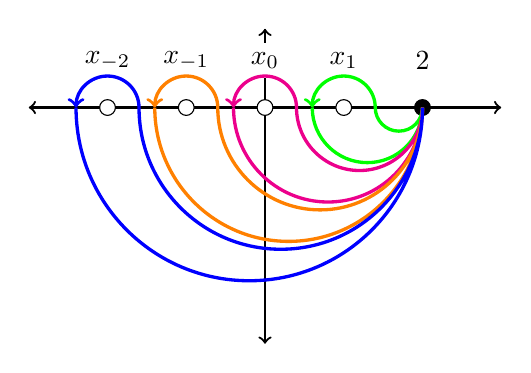
\begin{tikzpicture}
      \draw[<->, thick] (-3,0)--(3,0);
      \draw[<->, thick] (0,-3)--(0,1);

      \node at (2, 0.6) {$2$};
      \draw[fill=black] (2, 0) circle (0.1);

      \node at (1, 0.6) {$x_1$};
      \draw[fill=white] (1, 0) circle (0.1);
      \draw[<-, very thick, green] (0.6, 0) arc (180:0:0.4) arc (-180:0:0.3) arc (0:-180:0.7);

      \node[fill={white}] at (0, 0.6) {$x_0$};
      \draw[fill=white] (0, 0) circle (0.1);
      \draw[<-, very thick, magenta] (-0.4, 0) arc (180:0:0.4) arc (-180:0:0.8) arc (0:-180:1.2);

      \node at (-1, 0.6) {$x_{-1}$};
      \draw[fill=white] (-1, 0) circle (0.1);
      \draw[<-, very thick, orange] (-1.4, 0) arc (180:0:0.4) arc (-180:0:1.3) arc (0:-180:1.7);

      \node at (-2, 0.6) {$x_{-2}$};
      \draw[fill=white] (-2, 0) circle (0.1);
      \draw[<-, very thick, blue] (-2.4, 0) arc (180:0:0.4) arc (-180:0:1.8) arc (0:-180:2.2);
    \end{tikzpicture}
    \item
    The generators of $\pi_1(\mathbb C - \{-2, -1, 0, 1\}; 2)$ map to the
    generators of $\pi_1(\mathbb C - \{0, 1\}; 2)$ as follows:
    \begin{enumerate}[label={},align=left]
      \item[($x_1 \mapsto y_1$)]
      The map $f$ maps the right-half plane to the entire plane $\mathbb C$ in a
      conformal, injective way. So loops map to loops, and the interiors,
      exteriors, and orientations are preserved. Thus $x_1$ maps to a loop going
      around $f(1) = 1$ once in the positive direction.
      \item[($x_0 \mapsto y_0^2$)]
      Under $f$, a loop which is a circle around the origin maps to a
      circle which around the origin twice. Going from the base point to the
      circle along a path in the above diagram does not affect this.
      \item[($x_{-2} \mapsto \operatorname{id}$)]
      Here the image of the path under $f$ does not go around any holes in
      $\mathbb C - \{0, 1\}$, and so it deformation retracts to a constant path.
      \item[($x_{-1} \mapsto y_0^{-1}y_1y_0$)] Instead of considering the loop
      directly, instead consider the loop that goes from $2$ to $3$, then
      completes a positively oriented circle of radius $3$ around all holes,
      and then goes from $3$ to $2$. This is homotopic to the path
      $x_1x_0x_{-1}x_{-2}$. It's image goes from $4$ to $9$, then twice around
      a circle of radius $9$, and the back from $9$ to $4$, so it is homotopic
      to $(y_1y_0)^2 = y_1y_0y_1y_0$.
      Since $f_*$ is a homomorphism, \begin{align*}
          f_*(x_1x_0x_{-1}x_{-2}) &= y_1y_0y_1y_0 \\
          f_*(x_1)f_*(x_0)f_*(x_{-1})f_*(x_{-2}) &= y_1y_0y_1y_0 \\
          y_1y_0^2f_*(x_{-1})\operatorname{id} &= y_1y_0y_1y_0 \\
          y_0f_*(x_{-1})\operatorname{id} &= y_1y_0 \\
          f_*(x_{-1})\operatorname{id} &= y_0^{-1}y_1y_0.
      \end{align*}
    \end{enumerate}
    Therefore $f_*$ maps
    \begin{align*}
      x_{-2} &\xmapsto{f_*} \operatorname{id},\\
      x_{-1} &\xmapsto{f_*} y_0y_1y_0^{-1},\\
      x_0    &\xmapsto{f_*} y_0^2, \text{ and} \\
      x_1    &\xmapsto{f_*} y_1.
    \end{align*}
  \end{enumerate}
\end{proof}
\pagebreak
% -----------------------------------------------------
% Second problem
% -----------------------------------------------------
\begin{problem}{2} \text{} \\
  Define \begin{align*}
      S^1 &= \{z \in \mathbb C : |z| = 1 \} \text{ and}\\
      B^2 &= \{z \in \mathbb C : |z| \leq 1 \},
  \end{align*} and let $V_1$ and $V_2$ be two copies of $B^2 \times S^1$ whose
  boundries are identified to $S^1 \times S^1$.
  In $V_1$, let $D_1$ be the disk $B^2 \times \{ 1 \}$ with boundary canonically
  identified to $\partial B^2 = S^1$
  \begin{enumerate}[a.]
    \item Let $X$ be obtained from the disjoint union of $D_1$ and $V_2$ by
    gluing the boundary $\partial D_1 = S^1$ to $\partial V_2 = S^1 \times S^1$
    by the map $\phi\colon S^1 \rightarrow S^1 \times S^1$ defined by
    $\phi(u) = (u^a, u^b)$ for some $a, b \in \mathbb Z$. Compute the
    fundamental group of $X$.
    \item Let $L$ be obtained by the disjoint union of $V_1$ and $V_2$ by gluing the boundary $\partial V_1$ to $\partial V_2$ by the map \[
      \phi\colon \underbrace{S^1 \times S^1}_{\partial V_1}
      \rightarrow \underbrace{S^1 \times S^1}_{\partial V_2}
      \text{ which sends }
      \phi(u, v) = (u^av^c, u^bv^d)
    \] for some integers $a, b, c, d \in \mathbb Z$.
  \end{enumerate}
\end{problem}

\begin{proof} \text{} \\
  \begin{enumerate}[a.]
    \item
    First note that $D_1$ is homeomorphic to a disk and $V_2$ is homeomorphic to
    a solid torus. Thus $D_1$ deformation retracts to a point, and $V_2$
    deformation retracts to $S^1$.
    Therefore by van Kampen's theorem, we can write $\pi_1(X)$ as \begin{align*}
      \pi_1(X; [(x_1, x_2)]) &\cong
      \underbrace{\pi_1(D_1; x_1)}_{\mathbf{1}}
      \underbrace{*_{\pi_1(\phi(\partial D_1) \cap V_2; (\phi(x_1), x_2))}}_{*_\mathbb Z}
      \underbrace{\pi_1(V_2; \phi(x_1))}_{\mathbb Z} \\
      &\cong \mathbf{1} *_\mathbb Z \mathbb Z,
    \end{align*}
    There is only one choice of map (and thus homomorphism) for
    $i_A\colon \mathbb Z \rightarrow \mathbf{1}$, namely sending everything to
    the identity.
    Thus, it only remains to determine
    $i_B\colon \mathbb Z \rightarrow \mathbb Z$. Since $V_2 = B^2 \times S^1$
    deformation retracts to $S^1$ by the map $(b, s) \xmapsto{d} s$, and so
    $d \circ \phi(u) = d(u^a, u^b) = u^b$. Therefore the desired map is \[
      i_B(u) = d \circ \phi(u) = u^b
    \] so the fundamental group is simply the cyclic group \[
      \pi_1(X; [(\phi(x_1), x_2)])
      \cong \langle x; x^b = 1 \rangle
      \cong \mathbb Z/a\mathbb Z.
    \]
    \item Here we do a similar argument to part \textbf{a.}:
      By van Kampen's theorem, we can write \[
        \pi_1(X; [(x_1, x_2)]) \cong
        \underbrace{\pi_1(V_1; x_1)}_{\mathbb Z = \langle v_1; \rangle}
        \underbrace{*_{\pi_1(\psi(\partial V_1) \cap \partial V_2; (\psi(x_1), x_2))}}_{
          F_2 = \langle y_1, y_2; \rangle
        }
        \underbrace{\pi_1(V_2; \psi(x_1))}_{\mathbb Z = \langle v_2; \rangle}.
      \]
      Where $v_1$ and $v_2$ are loops around $S^1 \subset B^2 \times S^1$ in
      $V_1$ and $V_2$ respectively, and $y_1$ and $y_2$ are loops around
      $\partial B^2$, and $S^1$ respectively.
      \\
      Then the homomorphism
      $i_A\colon \langle y_1, y_2 \rangle \rightarrow \langle v_1 \rangle$ is given by
      \begin{align*}
        y_1 &\mapsto 1\\
        y_2 &\mapsto v_1,
      \end{align*}
      because the ``obvious'' deformation retract on $B^2 \subset V_1$ means
      that $y_1$ is nullhomotopic, and so maps to the identity. The loop $y_2$
      around $S^1 \subset \partial V_1$ maps into a single loop around
      $S^1 \subset V_1$.
      \\~\\
      Similarly, the homomorphism
      $i_B\colon \langle y_1, y_2 \rangle \rightarrow \langle v_2 \rangle$ is given by
      \begin{align*}
        y_1 &\mapsto v_2^b \\
        y_2 &\mapsto v_2^d,
      \end{align*} because given any loop
      $\alpha\colon [0,1] \rightarrow S^1 \times S^1$ can be decomposed and
      mapped to $\partial V_2$ by \[
        \alpha(t) = (\alpha_1(t), \alpha_2(t))
        \xmapsto{\psi} (\alpha_1^a(t)\alpha_2^c(t), \alpha_1^b(t)\alpha_2^d(t))
        \xmapsto{d} \alpha_1^b(t)\alpha_2^d(t).
      \]
      Therefore if $a_1$ is a curve that wraps around $\partial B^2$ once, then
      $\psi \circ \alpha_1\colon [0, 1] \rightarrow V_2$ is homotopic to a curve
      via the deformation retract $d$) that wraps around $S^1 \subset V_2$
      $b$ times.
      Thus the fundamental group has the presentation:
      \[
        \pi_1(X; [(x_1, x_2)])
        \cong \langle v_1, v_2; v_1 = v_2^a, v_2^b = 1 \rangle.
      \]
  \end{enumerate}
\end{proof}
\end{document}
